\toclesssection{Algorithms and Datastructures}

\begin{frame}{Algorithms and Datastructures}{Topics of this Lecture}
  \textbf{Topics of the Lecture:}
  \begin{itemize}
    \item
      \only<1-|handout:1>{Algorithms and Data Structures\\}
      \only<2-|handout:1>{
        Efficient data handling and processing\\
        $\ldots$ for problems that occur in practical \textbf{any} larger program / project
      }
    \item
      \textbf{Algorithm} $\hat{=}$ Solving of complex computional problems
    \item
      \textbf{Datastructure} $\hat{=}$ Representation of data on computer
  \end{itemize}
\end{frame}

%-------------------------------------------------------------------------------

\begin{frame}[t]{Example 1: Sorting}
  \hfill
  \qrcode[height=6em]{https://www.youtube.com/watch?v=kPRA0W1kECg}\\
  \vspace*{-1.5em}
  \begin{figure}[!h]
    \begin{center}
      \href{https://www.youtube.com/watch?v=kPRA0W1kECg}{
        \begin{adjustbox}{width=0.75\linewidth}%
          \def\MinSortDrawNumbers{0}
\begin{tikzpicture}
%Generate MinSort pattern
\foreach[count=\x] \h/\c in {
  1/MainBLight,%
  2/MainBLight,%
  3/MainBLight,%
  12/MainALight,%
  7/MainALight,%
  4/MainA,%
  6/MainALight,%
  10/MainALight,%
  8/MainALight,%
  15/MainALight,%
  14/MainALight,%
  5/MainALight,%
  11/MainALight,%
  9/MainALight,%
  13/MainALight%
} {
  \draw[fill=\c] (\x + 0.1, 0.0) rectangle (\x + 0.9, \h/2);
  \ifnum \MinSortDrawNumbers>0
    \draw (\x + 0.5, -0.5) node {\huge \h};
  \fi
}

% Draw play button
\draw[color=black, fill=Hell-Gruen]
  (8, 1.5) -- (8, 5.5) -- (10, 3.5) -- (8, 1.5);
\end{tikzpicture}%
        \end{adjustbox}
      }
    \end{center}
    \caption{%
      \href{https://www.youtube.com/watch?v=kPRA0W1kECg}{%
        Sorting with \textit{Minsort}%
      }%
    }%
    \label{fig:minsort_play}%
  \end{figure}
\end{frame}

%-------------------------------------------------------------------------------

\begin{frame}{Example 2: Navigation}
  \begin{columns}
    \begin{column}{0.55\textwidth}
      \begin{itemize}
        \item<2-|handout:1>
          \textbf{Datastructures:} How to represent the map as data?
        \item<3-|handout:1>
          \textbf{Algorithms:} How to find the shortest / fastest way?
      \end{itemize}
    \end{column}%
    \begin{column}{0.45\textwidth}
      \begin{figure}[!h]
        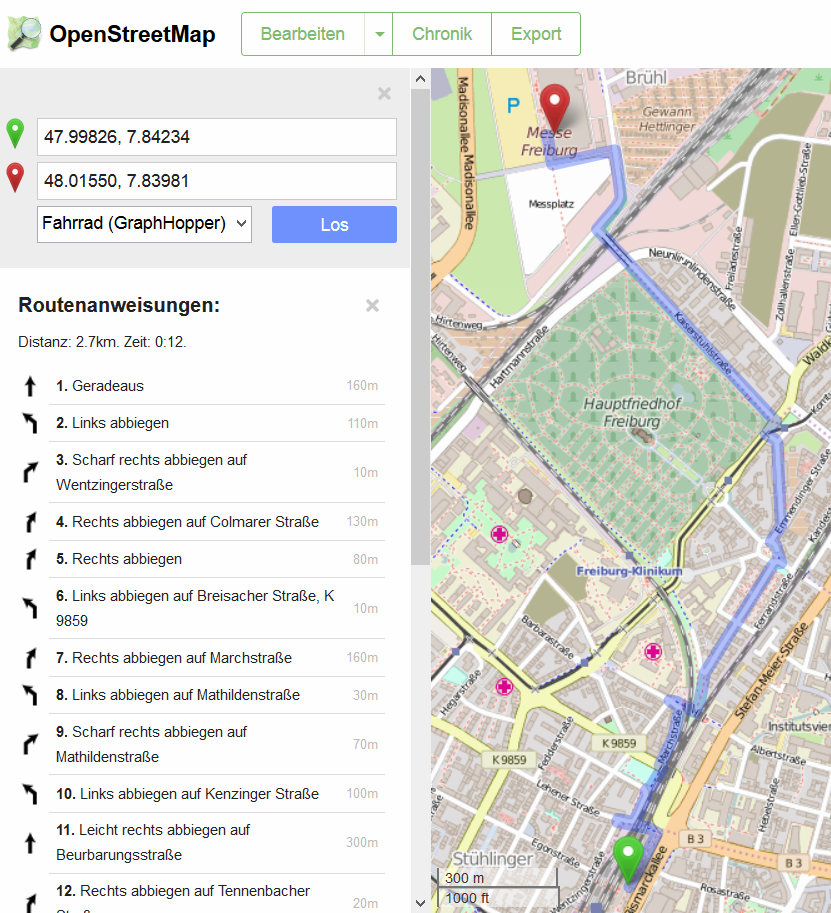
\includegraphics[width=\textwidth]
          {Images/Introduction/OpenStreetmap.png}
        \caption{Navigationplan \copyright\,%
          \href{http://openstreetmap.org/}{OpenStreetMap}%
        }%
        \label{fig:openstreetmap}
      \end{figure}
    \end{column}
  \end{columns}
\end{frame}
